\section*{Форматы входных и выходных файлов}

Входной файл представляет собой обычный текстовый файл, в котором содержится набор исходных строк текста (пример на рис. \ref{ife}).

\begin{figure}[H]
	\centering
	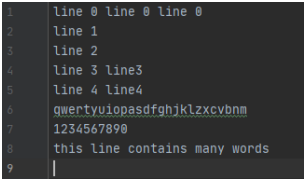
\includegraphics[width=0.6\linewidth]{photo/file_example}
	\caption{Пример входного файла}
	\label{ife}
\end{figure}

Выходной файл запысывается следующем формате:
\begin{itemize}
	\item вначале должны быть записаны исходные строки;
	\item потом должно быть записано название совершённой операции;
	\item потом должны быть записаны введённые данные и параметры;
	\item после чего уже должны быть записаны полученные строки.
\end{itemize}

Пример выходного файла на рис. \ref{ofe}.

\begin{figure}[H]
	\centering
	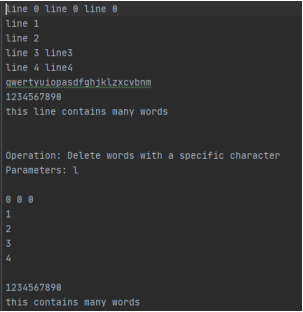
\includegraphics[width=0.6\linewidth]{photo/test.1.file}
	\caption{Пример выходного файла}
	\label{ofe}
\end{figure}